%================================== Geometrická optika =======================================================
\chapter{Geometrická optika}
\minitoc
\newpage
 \section{Úvod}
    Na několika přístrojích předvedeme aproximaci nazvanou \emph{geometrická optika}. Je to
    nejužitečnější aproximace pro praktickou konstrukci mnoha optických systémů a přístrojů.
    Geometrická optika je buď velmi jednoduchá nebo velmi komplikovaná.
    
    Abychom mohli pokračovat potřebujeme jeden geometrický vztah a to: máme-li trojúhelník s malou
    výškou $h$ a velkou základnou $d$, pak přepona $s$ je delší než základna (viz obr.
    \ref{FYZ:fig_trojuhelnik_optika}).  
    
    Tedy 
    \begin{equation}\label{FYZ:eq_triangle}
     \Delta \approx \frac{h^2}{2s}.
    \end{equation}
    To je celá geometrie, kterou je třeba znát, aby bylo možné diskutovat vznik obrazů pomocí
    zakřivených ploch.		         
    
    \begin{figure}
      \centering
      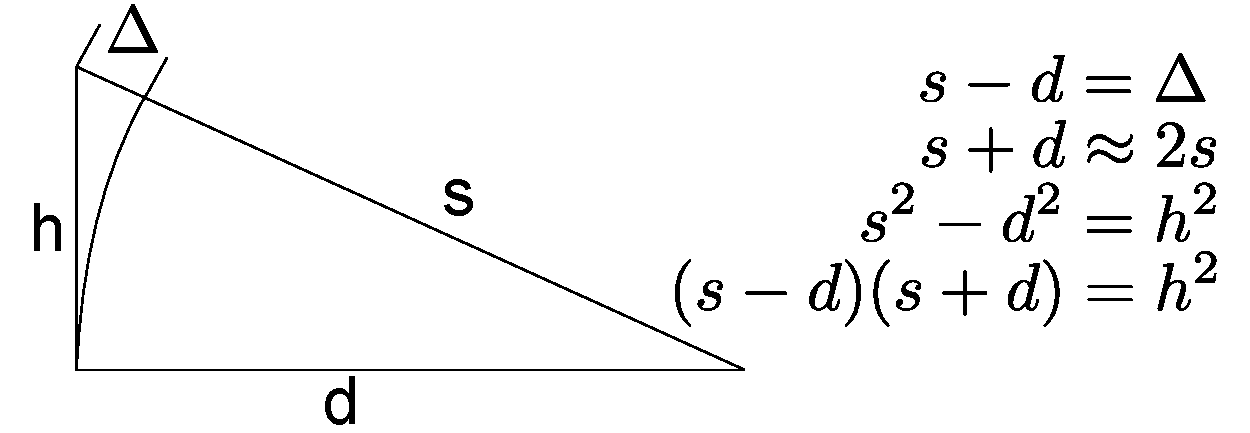
\includegraphics[width=\linewidth]{geom_optika_trojuhelnik.pdf}
      \captionof{figure}{Trojúhelník s malou výškou a velkou základnou }
      \label{FYZ:fig_trojuhelnik_optika}  
    \end{figure}

\printbibliography[heading=subbibliography]